% appendix/questions/time.tex
% SPDX-License-Identifier: CC-BY-SA-3.0

\section{What Time Is It?}
\label{sec:app:questions:What Time Is It?}

\begin{figure}[htb]
\centering
\resizebox{3in}{!}{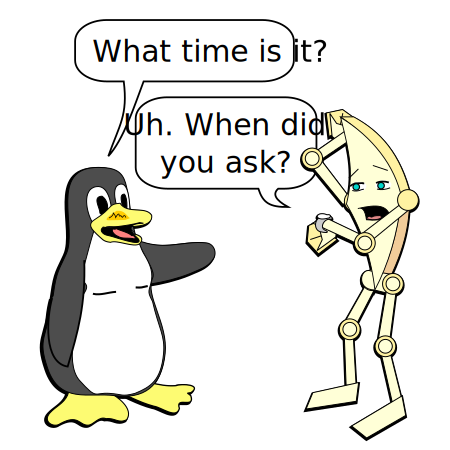
\includegraphics{cartoons/r-2014-What-time-is-it}}
\caption{What Time Is It?}
\ContributedBy{Figure}{fig:app:questions:What Time Is It?}{Melissa Broussard}
\end{figure}

A key issue with timekeeping on multicore computer systems is illustrated
by Figure~\ref{fig:app:questions:What Time Is It?}.
One problem is that it takes time to read out the time.
An instruction might read from a hardware clock, and might
have to go off-core (or worse yet, off-socket) to complete
this read operation.
It might also be necessary to do some computation on the value read out,
for example, to convert it to the desired format, to apply network time
protocol (NTP) adjustments, and so on.
So does the time eventually returned correspond to the beginning of
the resulting time interval, the end, or somewhere in between?

Worse yet, the thread reading the time might be interrupted or preempted.
Furthermore, there will likely be some computation between reading out
the time and the actual use of the time that has been read out.
Both of these possibilities further extend the interval of uncertainty.

One approach is to read the time twice, and take the arithmetic mean
of the two readings, perhaps one on each side of the operation being
timestamped.
The difference between the two readings is then a measure of uncertainty
of the time at which the intervening operation occurred.

Of course, in many cases, the exact time is not necessary.
For example, when printing the time for the benefit of a human user,
we can rely on slow human reflexes to render internal hardware and
software delays irrelevant.
Similarly, if a server needs to timestamp the response to a client, any
time between the reception of the request and the transmission of the
response will do equally well.

% @@@ Scheduling ticks

% @@@ Tickless operation

% @@@ Timers

% @@@ Current time, monotonic operation

% @@@ The many ways in which time can appear to go backwards

% @@@ Causality, the only real time in SMP (or distributed) systems
